% Copyright (C) 2014-2016 by Thomas Auzinger <thomas@auzinger.name>

\documentclass[draft,final]{vutinfth} % Remove option 'final' to obtain debug information.

% Load packages to allow in- and output of non-ASCII characters.
\usepackage{lmodern}        % Use an extension of the original Computer Modern font to minimize the use of bitmapped letters.
\usepackage[T1]{fontenc}    % Determines font encoding of the output. Font packages have to be included before this line.
\usepackage[utf8]{inputenc} % Determines encoding of the input. All input files have to use UTF8 encoding.

\RequirePackage[hyphens]{url}

% Extended LaTeX functionality is enables by including packages with \usepackage{...}.
\usepackage{amsmath}    % Extended typesetting of mathematical expression.
\usepackage{amssymb}    % Provides a multitude of mathematical symbols.
\usepackage{mathtools}  % Further extensions of mathematical typesetting.
\usepackage{microtype}  % Small-scale typographic enhancements.
\usepackage[inline]{enumitem} % User control over the layout of lists (itemize, enumerate, description).
\usepackage{multirow}   % Allows table elements to span several rows.
\usepackage{booktabs}   % Improves the typesettings of tables.
\usepackage{subcaption} % Allows the use of subfigures and enables their referencing.
\usepackage[ruled,linesnumbered,algochapter,noend]{algorithm2e} % Enables the writing of pseudo code.
\usepackage[usenames,dvipsnames,table]{xcolor} % Allows the definition and use of colors. This package has to be included before tikz.
\usepackage{nag}       % Issues warnings when best practices in writing LaTeX documents are violated.
\usepackage{todonotes} % Provides tooltip-like todo notes.
\usepackage{hyperref}  % Enables cross linking in the electronic document version. This package has to be included second to last.
\usepackage{listings} % Enables displaying source code
\usepackage{wrapfig} % Wraps text around figures
\usepackage{microtype} % Hyphenate words
\usepackage{graphicx} % To include images 
\usepackage[labelfont=bf]{caption} % make Listing and Figure bold
\usepackage[acronym,toc]{glossaries} % Enables the generation of glossaries and lists fo acronyms. This package has to be included last.

\graphicspath{ {graphics/} }


% Define convenience functions to use the author name and the thesis title in the PDF document properties.
\newcommand{\authorname}{Markus Gabriel} % The author name without titles.
\newcommand{\thesistitle}{Android SSL Vulnerability Analyzer} % The title of the thesis. The English version should be used, if it exists.

% Set PDF document properties
\hypersetup{
    pdfpagelayout   = TwoPageRight,           % How the document is shown in PDF viewers (optional).
    linkbordercolor = {Melon},                % The color of the borders of boxes around crosslinks (optional).
    pdfauthor       = {\authorname},          % The author's name in the document properties (optional).
    pdftitle        = {\thesistitle},         % The document's title in the document properties (optional).
    pdfsubject      = {Subject},              % The document's subject in the document properties (optional).
    pdfkeywords     = {a, list, of, keywords} % The document's keywords in the document properties (optional).
}

\setpnumwidth{2.5em}        % Avoid overfull hboxes in the table of contents (see memoir manual).
\setsecnumdepth{subsection} % Enumerate subsections.

\nonzeroparskip             % Create space between paragraphs (optional).
\setlength{\parindent}{0pt} % Remove paragraph identation (optional).

\makeindex      % Use an optional index.
\makeglossaries % Use an optional glossary.
%\glstocfalse   % Remove the glossaries from the table of contents.

% Set persons with 4 arguments:
%  {title before name}{name}{title after name}{gender}
%  where both titles are optional (i.e. can be given as empty brackets {}).
\setauthor{}{\authorname}{}{male}
\setadvisor{Priv.-Doz. Dr. techn.}{Edgar Weippl}{}{male}

% For bachelor and master theses:
\setfirstassistant{}{Georg Merzdovnik}{MSc}{male}
%\setsecondassistant{Pretitle}{Forename Surname}{Posttitle}{male}
%\setthirdassistant{Pretitle}{Forename Surname}{Posttitle}{male}

% For dissertations:
%\setfirstreviewer{Pretitle}{Forename Surname}{Posttitle}{male}
%\setsecondreviewer{Pretitle}{Forename Surname}{Posttitle}{male}

% For dissertations at the PhD School and optionally for dissertations:
%\setsecondadvisor{Pretitle}{Forename Surname}{Posttitle}{male} % Comment to remove.

% Required data.
\setaddress{Holubstraße 3/4/6}
\setregnumber{01326657}
\setdate{30}{06}{2017} % Set date with 3 arguments: {day}{month}{year}.
\settitle{\thesistitle}{\thesistitle} % Sets English and German version of the title (both can be English or German).
%\setsubtitle{Optional Subtitle of the Thesis}{Optionaler Untertitel der Arbeit} % Sets English and German version of the subtitle (both can be English or German).

% Select the thesis type: bachelor / master / doctor / phd-school.
% Bachelor:
\setthesis{bachelor}
%
% Master:
%\setthesis{master}
%\setmasterdegree{dipl.} % dipl. / rer.nat. / rer.soc.oec. / master
%
% Doctor:
%\setthesis{doctor}
%\setdoctordegree{rer.soc.oec.}% rer.nat. / techn. / rer.soc.oec.
%
% Doctor at the PhD School
%\setthesis{phd-school} % Deactivate non-English title pages (see below)

% For bachelor and master:
\setcurriculum{Software \& Information Engineering}{Software \& Information Engineering} % Sets the English and German name of the curriculum.

% For dissertations at the PhD School:
%\setfirstreviewerdata{Affiliation, Country}
%\setsecondreviewerdata{Affiliation, Country}


\begin{document}

\frontmatter % Switches to roman numbering.
% The structure of the thesis has to conform to
%  http://www.informatik.tuwien.ac.at/dekanat

\addtitlepage{naustrian} % German title page (not for dissertations at the PhD School).
\addtitlepage{english} % English title page.
\addstatementpage

\begin{kurzfassung}
Um sichere Kommunikation zu bieten nutzen viele Android Apps SSL/TLS. Vorhergehende Forschung konnte jedoch aufzeigen, dass viele Apps unsichere eigene Implementierungen der vom Android Framework angebotenen SSL-Certificate-Validierungskomponenten nutzen. Weiters wird SSL Certificate Pinning, eine Maßnahme, die von manchen Android Apps zur Erhöhung der Sicherheit eingesetzt wird, teilweise unsicher implementiert. Diese Schwachstellen ermöglichen es Angreifern Man-In-The-Middle Attacken durchzuführen und dadurch möglicherweise sensiblen Netzwerkverkehr zu modifizieren oder abzufangen.

Im Rahmen dieser Arbeit ist ein Web Service zur Analyse von Android Apps auf MITM-Schwachstellen entwickelt worden. Das Service analysiert hochgeladene APK Dateien zuerst statisch und führt die Apps dann in einer Testumgebung, in der eine MITM-Attacke ausprobiert wird, durch. Das entwickelte Web Service unterstützt anpassbare, automatisierte und verteilte Analyse und wird in dieser Arbeit präsentiert.
\end{kurzfassung}

\begin{abstract}
To provide secure network communication many Android apps use SSL/TLS. Previous research has however shown that there are many apps that use insecure custom implementations of the components for SSL certificate validation provided by the Android framework. Additionally, SSL certificate pinning, a measure employed by some Android apps to increase security, is sometimes implemented insecurely. These vulnerabilities enable an attacker to perform a Man-in-the-Middle attack and through this modify or eavesdrop on possibly sensitive network traffic. 

As part of this thesis I implemented a web service that analyses Android apps for such MITM vulnerabilities by first analysing the APK file statically and then running the app in a modified environment where a MITM attack is tried. This tool allows customizable, automated and distributed analysis and is presented in this thesis.
\end{abstract}

% Select the language of the thesis, e.g., english or naustrian.
\selectlanguage{english}

% Add a table of contents (toc).
\tableofcontents* % Starred version, i.e., \tableofcontents*, removes the self-entry.

% Switch to arabic numbering and start the enumeration of chapters in the table of content.
\mainmatter

\chapter{Introduction}

The rise of smartphones and tablets has lead to changes in the software world and poses new security challenges. One important issue is making sure that data transferred through the internet is protected, to avoid possibly sensitive data being intercepted. Apps are at an additional risk of being target of a Man-In-The-Middle attack, since they are often connecting to the internet via Wi-Fi and many different hotspots. This leads to an even increased importance of secure communication for apps. The general, widely used way to ensure secure communication is by using the Secure Sockets Layer (SSL).\\
The past has however shown, that there are many vulnerabilities in non-browser software caused by incorrect use of SSL. Georgiev et al. \cite{Georgiev} inspected SSL certificate validation in programming frameworks and SSL libraries, found vulnerabilities in important software such as cloud client APIs, merchant payment SDKs and web-service middleware and demonstrated that \textit{"SSL certificate validation is completely broken in many critical software applications and libraries"}. They attributed the root causes of these vulnerabilities to badly designed APIs of SSL implementations. \\
Regarding the more specific case of Android apps, an analysis of 35.000 free Android apps  for potential vulnerabilities against MITM attacks \cite{Fahl2012} revealed that 1.074 (8\% of the apps and 17,28\% of the apps that contain HTTPS URLs) of them contained code which is potentially vulnerable. In a subsequent manual audit of 100 apps, 41 of them proved to be vulnerable to Man-In-The-Middle attacks. The cumulative install base of these apps with confirmed vulnerabilities was estimated between 40 and 185 million users \cite{Fahl2013}. The causes for these vulnerabilities were custom implementations of SSL validation components provided by the Android framework and the resulting \textit{"central suggestion was to drastically limit custom SSL handling in apps"} \cite{Fahl2013}. \\
Such custom implementations were, however, required for use cases like testing the app without a valid certificate during development and improving security through certificate pinning. App developers that were having a need for these use cases did often not understand SSL well enough, had difficulties with SSL libraries and were guided by forum posts found on the internet. They therefore often implemented insecure custom SSL handling \cite{Fahl2013}. This fact lead to proposals to support the needed SSL related use cases via configuration files instead of requiring developers to use error-prone programmatic APIs \cite{Fahl2013,Tendulkar}. \\
With the release of Android 7 such a configuration-based approach is now offered via the Network Security Config \cite{NetworkSecurityConfig, Android7NetworkSecurityConfig}. The percentage of Android phones running on Android 7.0 or higher is, however, currently only at 9.5\% \cite{AndroidPlatformVersions}, nearly one year after its release in August 2016 \cite{Android7Release}. This leaves developers still having to use the old programmatic approach in case they want to target the majority of Androids userbase.

For apps targeting Android versions below 7.0, the recommendation of Georgiev at al. for developers to do more fuzzing and adversarial testing might be valuable \cite{Georgiev}. The aim of this thesis is to provide Android developers and security researches with an easy solution to perform adversarial testing. As part of the thesis a web service has been developed to automatically analyse uploaded Android Package Kit (APK) files for a range of SSL related vulnerabilities, including the ones mentioned earlier. Requirements for the web application are that it should allow customization of the scenarios to be analysed, be able to process a large number of APKs and be easy to set up.

The thesis is structured in the following way: Chapter 2 gives background information on the different threat scenarios that can be detected by the proposed analysis service. In Chapter 3  the state of the art and existing approaches to the analysis of Android apps for SSL vulnerabilities is explained. Chapter 4 gives a detailed overview of the architecture and implementation of the analysis service. Chapter 5 presents analysis results of 100 apps and Chapter 6 summarizes the thesis.


\chapter{Background and threat scenarios}

\section*{TrustManager}

A common vulnerability is the implementation of an insecure custom \texttt{javax.net.X509\-TrustManager}. It is the vulnerability analysed by most of the existing Android SSL vulnerability detection systems presented in the next chapter. The Android framework defines a \texttt{X509TrustManager} interface and provides existing implementations of this interface, which can be created by the \texttt{javax.net.ssl.TrustManagerFactory} class through for example the method \texttt{TrustManager.getDefaultAlgorithm()}. When creating a HTTPS connection using for example the \texttt{javax.net.ssl.HttpsURLConnection} class, a default implementation is used, but developers may also set their own \texttt{X509Trust\-Manager} class instead. This has legitimate use cases like the implementation of certificate pinning, which is a measure for further increasing SSL security and is described in a later section. Unfortunately, this possibility to customize SSL validation is often misused by developers running into SSL-related problems. They search the internet for advise and are often advised to simply set a TrustManager accepting all certificates. In other cases developers, who do not posses a certificate signed by a valid certificate authority for testing their applications, set their apps up to trust all certificates during development and then forget to remove this behaviour from their apps in production.
To make matters worse, many frameworks and libraries contain implementation classes of the \texttt{X509TrustManager} that accept all certificates. Some examples are \texttt{AcceptAllTrustManager}, \texttt{NonValidatingTrustManager} and \texttt{Permissivex509TrustManager} \cite{Fahl2012}.

This vulnerability allows attackers to perform a Man-in-the-middle attack, intercepting HTTPS requests from the app by providing any self-signed certificate with a matching hostname.

\section*{WebViewClient}

When using a WebView to display websites in an app, there are also similar pitfalls. A custom class can inherit from the \texttt{android.webkit.WebViewClient} and override the SSL error handling method \texttt{onReceivedSslError}. Often this method is implemented to ignore the SSL error and just calls \texttt{proceed} to show the website anyway. Like the TrustManager vulnerability such an implementation would allow an attack to intercept a HTTPS connection by supplying any self-signed certificate with a valid hostname. An analysis of 13.820 apps showed that 1.360 of them were statically vulnerable and confirmed the vulnerability for 645 of those apps with dynamic analysis \cite{Zuo}. 

\section*{HostnameVerifier}

Another problematic interface is \texttt{javax.net.ssl.HostnameVerifier}. This interface has a method \texttt{boolean verify(String hostname, SSLSession session)} which should check if a certificate is allowed for the host of the requested URL. A custom implementation of this class can also be set for a \texttt{HttpsURLConnection}. In their analysis of 35.000 apps, Fahl et al \cite{Fahl2012} found 453 apps implementing just the \texttt{org.apache.http.conn.ssl.AllowHostnameVerifier} class alone. \\
While accepting all certificates at least does not enable an attacker to intercept a SSL connection with any self-signed certificate, any valid certificate signed by a trusted certificate authority or its intermediaries - which an attacker can easily get for his own domain for example - is sufficient to perform a MITM attack.\\
Another related pitfall is the use in listing \ref{lst:hnsession}.
\begin{lstlisting}[language=Java,caption={Hostnameverifier ignoring session \cite{PinningSymposium}},label={lst:hnsession},frame=tb,columns=fullflexible]
HttpsURLConnection.setDefaultHostnameVerifier(new HostnameVerifier() {
    public boolean verify(String hostname, SSLSession session) {
        return hostname.equals("www.oursafebank.com");
    }
}
\end{lstlisting}
This does not check the SSLSession which contains the hostname of the server's certificate, but only checks the hostname of the URL requested by the client itself, therefore rendering the hostname verification useless. The issue here is, that developers assumed that the \texttt{hostname} parameter is the hostname of the server's certificate, which it is not.

\section*{Certificate pinning}

When using SSL in non-browser software like Android apps, it is often known with which hosts the program will communicate. This means that, in contrast to browser software, the certificate key distribution problem does not have to be solved with general mechanisms like certificate authorities. Instead of trusting all certificates signed by a set of trusted certificate authorities, pinning can be used. \textit{Pinning is the process of associating a host with their expected X509 certificate or public key} \cite{Pinning}. This is done by either adding the hosts certificate or public key to the application at development time or upon the first encounter of the certificate as Trust on First Use. The first version is of course safer. There at different levels at which pinning can be applied. Leaf Pinning is the process of pinning the leaf certificate or public key while CA Pinning only pins an intermediate or root certificate authority. The first approach is safer since only exactly one certificate is accepted. In contrast, the second approach allows for more flexibility and makes eventual changes to certificate settings easier \cite{Pinning}.

Regarding certificate authority breaches in the past, certificate pinning should be an earnestly considered measure to improve the security of an app. Some expamles of past breaches include the CA DigiNotar signing false certificates for widely used domain names like *.google.com and the CA Comodo's compromise of its UTN-USERFirstHardware certificate which was used to sign 85.440 HTTPS certificates directly and create 50 more intermediate CAs \cite{Arnbak}. The usage of certificate pinning seems, however, to not be widely applied, demonstrated by an analysis of 20 high profile apps such as GMail, Ebay and Instagram that revealed only 2 of them using SSL pinning  \cite{Fahl2012}.

Pinning can be implemented in Android by again setting a custom TrustManager with an appropriate \texttt{checkServerTrusted} method \cite{Oltrogge}, but it is also possible without doing this. The OkHttp library \cite{OkHttp} is an example for an Android library supporting certificate pinning without specifying a custom TrustManager.

\section*{getPeerCertificates bug}

Certificate pinning implementations sometimes contain errors, like using any pin for any host or only using pin validation for the first connection to a host and skipping the validation for all new connections to the host \cite{PinningSymposium}. These cases are not easily testable in my framework, however, one major bug regarding certificate pinning is. 

The getPeerCertificates bug renders pinning completely ineffective. It is based on the misuse of the \texttt{javax.net.ssl.SSLSession.getPeerCertificates()} and the \\
\texttt{javax.net.ssl.SSLSession.getPeerCertificatesChain()} methods. These methods return a list of certificates. Usually the first certificate is the leaf certificate, the second one is an intermediate CA certificate and the last one a root CA certificate. These certificates are, however just hints for a client which he may use for building a clean chain from the leaf certificate. Servers may include any certificates in this list, even certificates completely unrelated to each other. Now consider the case that this list is used for certificate pinning instead of the clean chain (the certificate chain that was verified and is trusted by an underlying SSL validation routine). An example is the code snippet from an old vulnerable version of the OkHttp Library \cite{OkHttp} in listing \ref{lst:okhttp} .
\\\\
\begin{lstlisting}[language=Java,caption={Vulnerable certificate pinning in old OkHttp library},label={lst:okhttp},frame=tb,columns=fullflexible]
for (int i = 0, size = peerCertificates.size(); i < size; i++) {
    X509Certificate x509Certificate = peerCertificates.get(i); 
    if (pins.contains(sha1(x509Certificate))) return; // Success!
}
\end{lstlisting}
Further assume that an attacker has access to the private key of a certificate authority trusted by the system, which is a threat scenario against which pinning should protect. To perform a MITM attack he can then build a leaf certificate for a requested host, set this leaf certificate as first element of the list, set his system-trusted root certificate as the second element and finally append the original list returned by the server to the list. The system will then validate the SSL connection since it trusts the root certificate of the attacker and the certificate pinning check will also succeed since the certificate list also contains the pinned certificate.

\section*{Not using HTTPS and SSLStripping}

Another even worse vulnerability than broken SSL verification is not using SSL when transferring sensitive data. An analysis of 100 apps found that 4 apps sent usernames and passwords in the clear during login, with also only one of them encrypting the passwords with a nonce \cite{Onwuzurike}. Another analysis of 90 apps, revealed that 10 of them sent passwords in the clear, with again only one password hashed - unsalted \cite{Gagnon}.

Additionally, there is also the possibility of a SSLStripping attack. A program is vulnerable to such an attack if a website, which contains HTTPS URLs, is loaded via HTTP instead of HTTPS. Since the website is therefore initially loaded over an insecure connection, an attacker in the middle can manipulate the website source sent to the client and exchange the "https://" prefixes of all the URLs in the website for "http://" prefixes, forcing subsequent requests to these URLs to be performed in plain-text. Especially Android apps using WebView might be vulnerable to SSLStripping, since users can follow links on the websites rendered in a WebView.

\section*{Other Threats}

Besides the mentioned threat scenarios, there are also other possible SSL vulnerabilities. An example is incorrect handling of expired certificates or certificates with unusual invalid field combinations like the ones produced with fuzzing or combinatorial methods \cite{Brubaker, Kleine}. While these cases are not specific to Android or mobile apps, it is useful to have tool support to also test for such vulnerabilities on the Android platform. For this reason, the Android SSL Analyzer Service allows users to set their own leaf and root certificates to be used during analysis. 

\chapter{Existing approaches}

An initial step towards automated analysis for SSL vulnerabilities has been made by Fahl et al. \cite{Fahl2012} who developed a static analysis tool MalloDroid with which they analysed the 35.000 Android apps mentioned earlier. MalloDroid checks first if the app actually requires the internet permission to sort out apps that do not even connect to the internet. 
It then searches the APK for custom \texttt{X509TrustManager}, \texttt{HostnameVerifier} or \texttt{WebViewClient.onReceivedSslError()} implementations. \\
Mallodroid also collects the URLs found in the apps code to categorize the app as either HTTP only, mixed-mode (HTTP and HTTPS) or HTTPS only. For each discovered HTTP URL Mallodroid tries to connect via HTTPS in order to find out if there are any connections with could be made more secure by upgrading them to HTTPS. Additionally, mixed HTTP and HTTPS URLs could hint to possible SSLStripping vulnerabilities. \\
Since MalloDroid does not dynamically analyse the apps, it can not automatically verify vulnerabilities, but only guide further manual analysis.

A fully automated analysis framework for detecting apps with a \texttt{X509TrustManager} accepting all certificates is SMVHunter
\cite{Sounthiraraj}. The techniques employed by this tool can be summarized as follows: Static analysis collects the names of the activities containing uses of a custom TrustManager. These will then be used as entry points for dynamic analysis. Another type of static analysis collects the input fields of each of the apps activities and determines their type (for example Integer Input Field or URL Input Field). If entry points were found, dynamic analysis is performed. The app to analyse is installed in an emulator that channels its HTTP/S traffic through a Man-In-The-Middle proxy that uses a self-signed root certificate. Then each activity from the entry points is started and the input fields with their types are used to generate smart input to fill the input fields displayed in the activity. All other clickable fields of the activity are then clicked to eventually cause actions leading to HTTPS requests being made. After this UI automation, the logs are analysed to find if any HTTPS connections were accepted by the app.\\
SMVHunter is designed as system for large-scale analysis of Android apps and runs apps in parallel on multiple emulators.\\
My Android SSL Analyzer Service is heavily based on SMVHunter, reusing its open-sourced code \cite{SMVHunterGit} for static analysis and smart input generation and employing similar techniques during dynamic analysis.

A similar automatic framework is described in \cite{Zuo}, with the difference that this system tries to find a SSL vulnerabilitiy in Android WebViews.

\cite{Gagnon} proposed an approach that allows testing for more vulnerabilities than SMVHunter does. It supports different scenarios by using different certificates in the Man-In-The-Middle proxy. Their implementation does however not perform static analysis, but instead requires user input to an app in order to trigger HTTPS requests and their scenario for detecting incorrect host verification requires obtaining a valid certificate for the domain to which the request is made. This may be possible for developers testing their own apps, but not for security researchers testing other apps. My framework supports some of the scenarios and other similar scenarios without requiring users to own any valid certificates. 

\cite{Conti} take a different approach than SMVHunter and the other listed analysis frameworks by creating an app for on-device analysis for the same MITM vulnerability - apps accepting all certificates. This app is intercepting HTTPS traffic and serving fake certificates during normal execution of apps by the user.  In contrast to the other analysis-only tools, this tool can also be used to protect users by not allowing the execution of apps found out to be vulnerable.

To recap, the existing approaches either focus on single threat scenarios or require user interactions with the app to analyse. To the best of my knowledge, a fully automated tool that tests for all the threat scenarios listed in the previous chapter does not exist. I also could not find an existing system that determines if an app uses certificate pinning.



\chapter{Architecture}

\section*{General Architecture}

The Android SSL Analyzer project consists of three subprojects: the webapp, the static analysis task and the dynamic analysis task. Celery \cite{Celery}, an asynchronous task queue framework based on distributed message passing, is used to perform the static and dynamic analysis tasks asynchronously on possibly multiple computers. For this, Celery uses an underlying message broker for distributing the tasks to workers. In the Android SSL Analyzer Service, RabbitMQ \cite{RabbitMQ} is used as message broker. Workers initialize Celery with the URL of the RabbitMQ message broker and tasks are then distributed by the RabbitMQ server to an available worker that supports the task type - either static analysis or dynamic analysis. This architecture supports scalable, distributed, large-scale analysis. The number of static and dynamic analysis workers can be chosen depending on the analysis speed requirements and available computing resources. In contrast to SMVHunter, where large-scale analysis of Android apps is supported by running multiple emulators in parallel on a single computer, this architecture does add overhead, but enables analysis on a much larger scale, provided the availability of enough computing resources.

The task results are returned using again RabbitMQ as message broker, but instead of using the Celery support for using RabbitMQ as result backend, they use Flask-socketio's \cite{Flask-socketio} support for emitting results from external processes to websockets. To explain this in more detail: The webapp, which is written using the Flask \cite{Flask} microframework, communicates analysis results to its clients via Websockets using the Flask-socketio plugin. This plugin also allows external processes like Celery tasks to send results to the clients through the existing websockets between the clients and the webapp. This is done by initializing the Socketio client instances of the tasks and the Socketio server instance of the webapp with the RabbitMQ server URL. Results emitted by the tasks will then be sent to the webapp server via the RabbitMQ message broker and then from the webapp automatically to the clients via the existing websockets.\\
In contrast to using standard Celery result backends like RabbitMQ or SQL databases, this approach avoids either excessive polling of all the states of the single tasks from the client or complex combined polling of the tasks states in single poll requests from the client.

The three subprojects share a \texttt{common} subproject that contains data models that can be used to communicate with the MySQL database that holds scenario settings and certificates used during analysis. The common subproject further contains HTML templates and code for creating HTML for single analysis results.  These templates are needed to create HTML for the task results on the tasks directly instead of in the server, since the tasks themselves emit the results to the clients websocket as described earlier.  

To make the deployment and setup of the Android SSL Analyzer easy, Docker \cite{Docker} is used. Docker files to build dynamic analysis worker, static analysis worker and webapp containers are provided. Since all the required dependencies are isolated in a container, users don't have to worry about conflicts caused by different environments. A docker-compose configuration file \cite{DockerCompose} is further provided to allow running the whole service with the single command \texttt{docker-compose -f docker-compose-local.yml up -{}-build}. To deploy the Android SSL Analyzer Service on multiple machines, the IP of the manager machine, which uses the \texttt{docker-compose-manager.yml} configuration file, has to be set in the \texttt{common.config.py} file. On other machines one can then execute docker-compose with the \texttt{docker-compose-workers.yml} configuration file to run a static and dynamic analysis worker on the machine. These workers will then connect to the manager at the configured IP.

\section*{Webapp}

The web service is implemented as simple Flask webapp. Users can create new accounts and log in to adjust the settings influencing the analysis. The settings are grouped in scenarios and certificate settings.

A scenario represents a check for a specific threat. It can be enabled or disabled, which results in it either being included in the analysis process or not. A scenario has a vulnerability type that determines in which cases the dynamic analysis for this scenario will be run. The vulnerability type is HostnameVerifier, TrustManager, WebViewClient, Selected Activities, HTTPS URLs Heuristic, HTTP URLs Heuristic or HTTP and HTTPS URLs Heuristic. If one of the first three vulnerability types is used, dynamic analysis for this class will only be run if the static analysis has found a custom implementation of the respective class. All activities using these custom implementations will be analysed. The Selected Activities type will let the user choose during runtime which of all the apps activities should be analysed. The last three types are based on a heuristic for finding activities in which HTTPS or HTTP Strings are used. Only these activities will then be analysed during dynamic analysis. A scenario further has a MITM certificate field that specifies the certificate settings to be used by the MITM proxy when intercepting traffic.

\begin{figure}
\caption{Scenario view}
\label{fig:scenario}
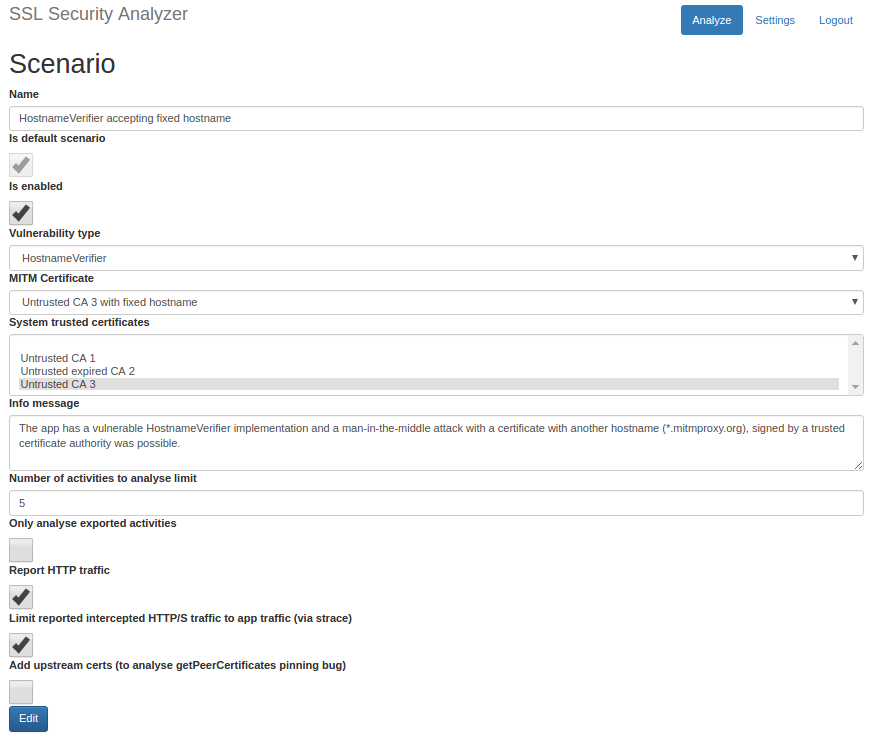
\includegraphics[width=\textwidth,height=0.5\textheight]{scenario_new.png}
\end{figure}

\begin{figure}
\caption{Certificate view}
\label{fig:cert}
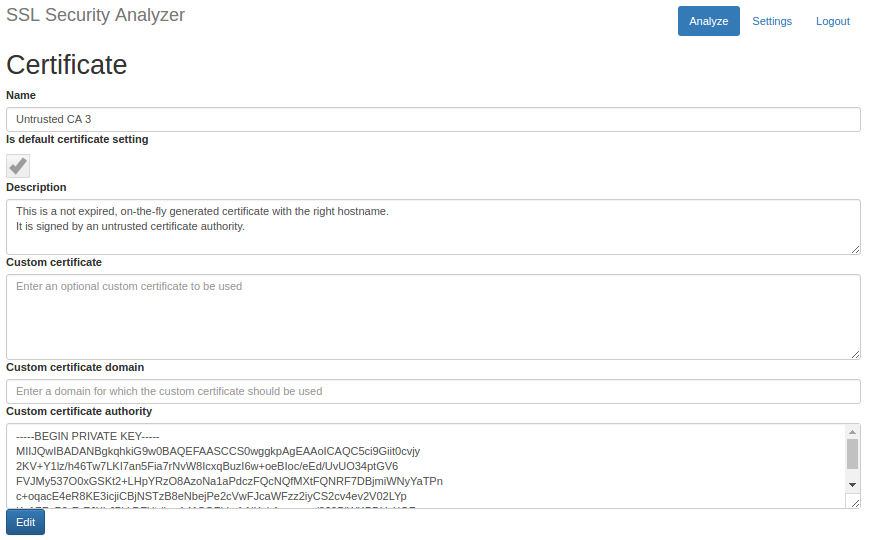
\includegraphics[width=\textwidth,height=0.4\textheight]{certificate_new.png}
\end{figure}

Another system trusted certificates list field contains all certificate settings whose certificate authority should be installed as system trusted on the emulator on which the analysis will be performed. Then there is a field for specifying the maximum number of activities to analyse, which helps limiting the duration of the dynamic analysis for apps with many activities. Finally, there are three flags with whom users can control if intercepted HTTP traffic should also be reported, if Android system traffic should not be reported (also called the strace option, for reasons explained in a later section) and if the original certificates of a requested host should be included as peer certifcates in order to allow checks for the getPeerCertificates bug.

The MITM certicate and system trusted certificates fields are a reference to a certificate object. Such an object can either have the custom certificate or the custom certificate authority field set. A certificate in PEM format containing a private and a public key can be given as input for these fields and will then be used during analysis instead of the default custom certificate authority which the MITM proxy uses to generate certificates on the fly. The "custom certificate domain" field can be used to only serve the custom certificate for the given domain.

The Android SSL Analyzer Service has a range of default scenarios and certificates for common analysis cases. These include among others
\begin{itemize}
\item TrustManager accepting untrusted CA: Uses default MITM proxy CA and has TrustManager as vulnerability type. This scenario can find custom TrustManager implementations accepting all certificates with a correct hostname.
\item HostnameVerifier accepting fixed hostname: Uses a custom certificate with a fixed hostname (".mitmproxy.org"), signed by a certificate authority that is added as system trusted certificate and uses the HostnameVerifier type. This allows detection of vulnerable HostnameVerifier implementations.
\item App accepting fixed trusted CA (No pinning): Uses a custom certificate authority in both the MITM proxy and as system trusted certificate. The scenario also has the strace option enabled since otherwise all system traffic could also be successfully intercepted leading to false positives in the result.  With this scenario users can detect if certificate pinning is (not) used.
\item App accepting peer certificates (No pinning): Has the same settings as the previous scenario, with additionally the getPeerCertificates flag set. If the previous scenario shows no vulnerability, but this scenario does, then the app has a getPeerCertificates vulnerability.
\item WebViewClient accepting untrusted CA: Has the same settings as the "TrustManager accepting untrusted CA" scenario with only WebViewClient as vulnerability type and tests for WebViews ignoring SSL errors and accepting all certificates.
\end{itemize}

An app analysis can be started by connecting to the websocket of the web application and uploading one or more APKs. The state of the analysis is displayed in a matrix view, with each row containing information about a scenario, possibly grouped again in subrows with dynamic analysis results for each activity of the scenario that was or will be analysed. As soon as static or dynamic analysis tasks are finished the corresponding rows in the matrix are updated. Figure \ref{fig:matrix} in the next chapter shows an example of the analysis results matrix view.

\section*{Static analysis}

For each APK to be analysed, a static analysis task is started with the name of the APK and the username of the user requesting the analysis as parameters. The static analysis task first retrieves the APK file from the webapp and then dissassembles the APK using Apktool \cite{Apktool}. This tool reverse engineers an APK file to convert the source code from its original Dalvik Executable (.dex) format into a higher level, human readable representation, called Smali, which is easier to work with during static analysis. Disassembly to Smali is chosen over decompilation to Java code since it is faster and cannot be be hindered by obsfuscation techniques \cite{Sounthiraraj}.

The next static analysis step is checking the Android Manifest of the app for an INTERNET permission request. If an app does not request this permission, it can not connect to the internet and further analysis is therefore unnecessary, since it can not be vulnerable. For the core of the static analysis I then reused the code of SMVHunter and extended it to fit my use cases. To find possible vulnerabilities, all Smali files are inspected for custom implementations of the X509TrustManager. I extended the inspections to also check for the other two types of custom implementations. The program searches for the following strings in the Smali files to find custom implementations:
\begin{itemize}
\item \texttt{.implements Ljavax/net/ssl/X509TrustManager;}
\item \texttt{.implements Ljavax/net/ssl/HostnameVerifier;}
\item \texttt{.super Landroid/webkit/WebViewClient;}
\end{itemize}
In the case of the WebViewClient, the program also checks if \texttt{onReceivedSslError} can be found in the smali file, since only WebViewClient classes overriding this method are possibly vulnerable.\\
SMVHunter's own implementation further compared the code of the TrustManager's \texttt{checkServerTrusted} method to the code of a range of vulnerable implementations. The Android SSL Analyzer Service does not perform such checks, neither for the TrustManager nor for the other classes. This means that all custom implementations will be analysed dynamically. In contrast, SMVHunter will only analyse apps with definitely vulnerable implementations to make sure that these implementations are actually used during runtime and are not just classes used for example only during testing. My approach has worse performance since it analyses more apps dynamically, but allows detection of other unknown vulnerable implementations.\\
To avoid simply testing all activities of a possibly vulnerable app during dynamic analysis, a set of entry points is created during static analysis to limit the activities to analyse dynamically to those that use a custom implementation of the mentioned classes. This is done by building a method call graph of the application and tracing the invocations of the vulnerable methods back to activities. The method call graph is generated by creating nodes for all methods and setting the node's children, and inversely the children node's parents, to all the methods that are invoked by the method of the node. One can then simply traverse the method call graph starting from the methods of the custom implementations following their parents and so on. Since some methods are only called by system code, the algorithm follows the parents of the constructor of the method's class in cases where the method itself is never called. If a method and also the corresponding constructor both have no parents, then we have arrived at a root of the graph and check if the class of this root node is an activity by searching the manifest of the app for an activity element with the same class name. Other possible entry points like services or content providers are not accepted, since dynamic analysis is only based on jumping to an activity entry point. 

If the Android SSL Analyzer Service used only the possible entrypoints explained up to this point,  then we would have the problem that our analysis would be limited to apps with the mentioned custom implementations. Since it is, however, possible that certificate pinning is implemented without a custom TrustManager and since we might just want to check if an app makes clear-text requests, a more general way of finding entry points is needed. The Android SSL Analyzer Service offers two types of general entry point selection. A manual one, presenting the user with all the activities of the app and allowing him to choose the ones to analyse, and the automated, heuristic approaches of using all activities that contain HTTP URLs, HTTPS URLs or URLs of both types as entry points. Obviously, the second approach might cause some false positive entry points, since not all methods using HTTP/S URLs will actually cause HTTP/S requests. I assume, however, that most will do.

To implement these URL entrypoints, we can reuse the method call graph from the existing static analysis, we only have to find methods in which these URLs are used and can then trace their invocations back to their activities using the existing method call graph traversal algorithm. 

\begin{algorithm}
\caption{Get all methods in which HTTPS strings are set.}
\label{alg:http}
$results \gets \emptyset$\;
\For{smaliFile $\in$ allSmaliFiles()}{%
	\For{method $\in$ methodsOf(smaliFile)}{%
		pattern = "const-string .*, \textbackslash "(https://.*)\textbackslash ""\;
		matches = findPatternMatches(pattern, method)\;
		\If{matches}{%
			$results \gets results \cup method$\;
		}
	}
}
\end{algorithm}

Algorithm \ref{alg:http} illustrates a simple way to get all the methods in which HTTPS strings are set.
The \texttt{const-string} instruction assigns a String constant to a temporary variable. Therefore this code will return all methods in which a string containing "https://" is set. The methods will often be constructors for instance variables or normal methods for local variables. The presented algorithm does not return the methods in which these variables will further be used, but only those in which they are initialized or set to another string constant. This causes some further false positives if objects with URL string fields are created, but their methods using these fields are not called. On the other hand, the use of Dependency injection frameworks will lead to false negatives, since constructors will not be called in the context of the activity.

One additional issue with the presented algorithm is that static URL string fields can not be used to create entry points. This is due to the fact, that static fields are initialized in the \texttt{<clinit>} class initialization method, which is called directly by the JVM and can therefore not be traced back to an activity via the method call graph. The adjusted algorithm \ref{alg:static_http} solves this.

\begin{algorithm}
\caption{Get all methods and static fields with HTTPS strings.}
\label{alg:static_http}
$results \gets \emptyset$\;
\For{smaliFile $\in$ allSmaliFiles()}{%
	\For{method $\in$ methodsOf(smaliFile)}{%
		\uIf{nameOf(method) $=$ "<clinit>"}{%
			pattern = "const-string (v[\^{},]*), \textbackslash "(https://.*)\textbackslash "\textbackslash s*sput-object (v[\^{},]*), (.*)"\;
			matches = findPatternMatches(pattern, method)\;
			\For{var1, url, var2, field $\in$ matches}{%
				\If{var1 $=$ var2}{%
					$results \gets results \cup field$\;
				}
			}
		}
		\uElse{%
			pattern = "const-string .*, \textbackslash "(https://.*)\textbackslash ""\;
			matches = findPatternMatches(pattern, method)\;
			\If{matches}{%
				$results \gets results \cup method$\;
			}
		}
	}
}
\end{algorithm}

This algorithm returns the names of static fields containing HTTPS strings in addition to the names of methods with HTTPS strings. The old algorithm is extended to handle \texttt{<clinit>} methods in a special way.\\
The class initialization method is searched for \texttt{const-string} instructions with HTTPS URLs followed by \texttt{sput-object} methods. This is the way static fields are assigned in most cases. An Smali example of such an assignment is presented in listing \ref{lst:static_smali}. A case which is not supported is for example building static strings as concatenation of multiple non-final strings, since this produces a different set of instructions. The check for var1 $=$ var2 is an additional safeguard to guarantee that the same temporary variable which contains the constant HTTPS string is used in the \texttt{sput-object} instruction.\\
With this adjustment the original static analysis has to also be adjusted to allow static fields as leafs for the method call graph. When building the method call graph, additionally to the method invocations of a method, all \texttt{sget-object} instructions of a method are inspected to add their fields as children, and inversely the method as their parents, in the method call graph.

\begin{lstlisting}[caption={Smali code for static field initialization},label={lst:static_smali},frame=tb,columns=fullflexible,breaklines]
.method static constructor <clinit>()V
	.locals 1

	.prologue
	.line 5
	const-string v0, "https://www.amazon.de"
	sput-object v0, Lcom/example/markus/httpsstringstestapp/ExternalStrings;->url:Ljava/lang/String;

	return void
.end method
\end{lstlisting}

To support the manual activity selection alternative, the list of all activies is retrieved through the single method \texttt{get\_activities()} of the Androguard reverse engineering framework \cite{Androguard}.

A next step is the generation of smart input. I took the exactly same approach as SMVHunter. For all \texttt{EditText} elements in the layout of an activity, the element ID and an eventual input type annotation are extracted. Input type annotations can be added by developers to control the keyboard that is shown to the user on selection of an input field. Examples are \texttt{TYPE\_CLASS\_PHONE} for fields that expect phone numbers, \texttt{TYPE\_CLASS\_VARIATON\_EMAIL\_ADDRESS} for email addresses and \texttt{TYPE\_CLASS\_NUMBER} for numbers. If there is no type annotation, the apps code is searched for variables referencing the EditText by ID and those variables are tracked up to cast operations. The input type for the corresponding field is then set to the type to which the variable is casted. The resulting assignment of input IDs to input types can then be used later in dynamic analysis to insert text into the input fields based on a predefined mapping of each input type to example input text . A detailed description of the smart input generation technique can be found in \cite{Sounthiraraj}.

At the end, the static analysis task retrieves the enabled scenario settings of the user and joins the scenario settings and static analysis results into concrete scenarios based on their vulnerability types. For each of these concrete scenarios a dynamic analysis task is started. So only scenarios for whose vulnerability type corresponding entry points have been found during static analysis will be dynamically analysed. The static analysis results are additionally used to render HTML which will be sent to the client via the previously explained websocket architecture to update the analysis result matrix view. Further, if there are any enabled scenario settings that require manual activity selection, then the static analysis and smart input results are saved in the MySQL database so that they can be retrieved later if the user has selected the activities to analyse.

\section*{Dynamic analysis}

A dynamic analysis task is started with the apk name, the scenarios to analyse, the smart input results and the username as parameters.
The task then performs the following actions:
\begin{itemize}
\item Start the emulator
\item Install the APK
\item Start the app
\item For each activity
	\begin{itemize}
	\item Install system trusted certificates
	\item Start MITM proxy
	\item Possibly strace app
	\item Run UI automation
	\item Analyse logs
	\end{itemize}
\end{itemize}
The stock android emulator provided as part of the Android SDK is used. The \texttt{minSdkVersion} and \texttt{targetSdkVersion} attributes from the Android Manifest, which where determined in the static analysis, are considered to choose an emulator with a fitting API level. Usually, only a limited set of API levels will be available on the docker image of the dynamic analysis task. Therefore the emulator with the lowest available API level in the range of minSdkVersion and targetSdkVersion will be chosen. The emulator is initialized to send traffic to the MITM proxy by setting the URL and port of the proxy with the \texttt{-http-proxy} option.\\
Since only a single dynamic analysis task worker runs in a docker container and the emulator is started and shutdown for every task, there is no need for the management of parallel emulators. In contrast, SMVHunter needs to manage an emulator pool and detect emulators which switch to an "offline" state and become unresponsive when run for a longer period of time \cite{Sounthiraraj}. Sometimes there were, however, emulator freezes during dynamic analysis. These failures were addressed by setting a timeout of 10 minutes for a dynamic analysis task and retrying a timed out task once.

To install the APK and start the app, simple Android Debug Bridge (adb) \cite{Adb} commands are used.

The next step is the installation of the system certificates of the scenario in the emulator. The root certificates trusted by the Android system are located in the \texttt{\char`\\system\char`\\etc\char`\\security\char`\\cacerts} folder. The filenames of the certificates are the hashes of their subject name. To add a PEM system certificate set by the user, the public key is extracted, the hash of the subject name is built, the certificate with the public key part is saved in a file with the hash as name and then the file is pushed to the emulator via adb. To allow pushing files to the \texttt{\char`\\system} folder, the emulator has to be started with the \texttt{-writable-system} option and (re-)mounted as root user.\\
An example sequence of commands to add a certificate as system trusted on Android is the following:
\begin{lstlisting}[caption={(Specific) commands for adding system trusted certificate},label={lst:static_smali},frame=tb,columns=fullflexible,breaklines]
openssl x509 -inform pem -in /files/tmp/certs/installed_cert.pem -out /files/tmp/certs/installed_cert.crt
openssl x509 -in /files/tmp/certs/installed_cert.crt -subject_hash_old -noout
openssl x509 -in /files/tmp/certs/installed_cert.crt >> c7008313.0
openssl x509 -in /files/tmp/certs/installed_cert.crt -text -fingerprint -noout >> c7008313.0
adb -s emulator-5554 root
adb -s emulator-5554 remount
adb -s emulator-5554 push c7008313.0 /system/etc/security/cacerts
\end{lstlisting}

As next step, the Man-In-The-Middle proxy is started. Mitmdump \cite{Mitmproxy} is used as proxy in the Android SSL Analyzer Service. It allows setting custom certificates, custom certificate authorities and certificate domains that work as described in the webapp section. Furthermore scripts that are executed on certain events like HTTP/S requests and have access to request information can be set. Such a script is used to write the target host and ip of a request with an established TLS connection to a log file. To detect plain text requests, all requests with HTTP as protocol are also written to a log file. This logging approach using scripts avoids analysis of possibly unclear default proxy logs which might require complex and error-prone parsing.

In the webapp section explaining the scenario settings, an option that specifies if Android system traffic should not be reported was mentioned. This option exists, since the MITM proxy logs all requests from the emulator and can not differentiate between different apps and/or the Android system. To limit the reported traffic to only the one app to be analysed, the strace linux tool can be used. This command can attach to a process and report the system calls made by the process. If the current scenario has the strace option set, then the process of the app to analyse is determined by searching for the apps package name and then stracing all \texttt{connect} system calls of this process.\\
Later when analysing the logfiles, only those IPs of the MITM proxy logs that match any IP received from the strace logs are returned as IPs that could be successfully intercepted.\\
The strace option is not enabled per default, since it slows the traced process down. If a scenario has the same certificate authority set as MITM proxy CA and also installed in the emulator as system trusted, then the strace option should be activated, since all system traffic would otherwise also be intercepted. Therefore all default pinning scenarios use this option. Additionally scenarios that report HTTP traffic should also use this option.

After the environment has been set up, the activity is started and UI automation is performed. Each EditText displayed in the activity is filled with the correct smart input. Then all clickable views of the activity are tapped. The AndroidViewClient library \cite{AndroidViewClient} is used get all the UI elements on the screen and to make text and tap inputs without having to deal with the coordinates of the elements or similar UI related issues. If, after a tap, the keyboard is shown, then the back button is pressed to make the keyboard disappear so that it does not interfere with further taps on UI elements. After a tap the analyzer service further waits and then checks if the current window has changed. If this is the case, the back button is pressed to get back to the old window. Since there are "non-cancellable" and other UI elements that may disable the back button effect temporarily \cite{Sounthiraraj}, the current window state is checked again to determine if  the back button click was successful. If this was not the case, two other "Enter" events are generated to try to close these dialogs.\\
One thing to note is, that while the Android SSL Analyzer Service can also analyse WebViews it does not perform crawling of the WebView's displayed website in case the URL was not a HTTPS URL. This is an approach taken by another framework to detect SSL vulnerabilities in WebViews \cite{Zuo}. Since WebViews loading HTTP URLs are vulnerable to SSLStripping and the Android SSL Analyzer Service can report HTTP connections, such techniques are not required.\\
When UI automation for an activity is finished, the logs are analysed for successful HTTP/S connections as described earlier. The results of the activities' analysis are sent to the client's websocket to refresh the displayed analysis state.

\chapter{Evaluations}

To demonstrate the functionality of the Android SSL Analyzer Service and to gather some information about the current state of SSL vulnerabilites in Android apps I performed an analysis of 100 apps.

The 100 top apps in the Google Play store, localized to Austria, were analysed. The apps were tested for the 4 default scenarios "TrustManager accepting untrusted CA", "HostnameVerifier accepting fixed hostname", "App accepting fixed trusted CA (No pinning)" and "WebViewClient accepting untrusted CA". A more detailed description of these scenarios can be found in the webapp section of chapter 4. The apps were downloaded from the Google Play store on an x86 emulator running Android 5.0. This was required since the Android SSL Analyzer Service only uses x86 emulators because of their hardware acceleration support and APKs using ARM native libraries can not be analysed. The analysis was run on a Lenovo Thinkpad T440s laptop running the manager docker-compose applications (the webapp, RabbitMQ and MySQL) and the workers docker-compose applications (one dynamic and static analysis worker each) and a desktop PC with an AMD FX-6200 processor running another set of workers docker-compose applications. The analysis was completed after about two hours. 

The results were as follows
\begin{itemize}
\item 10 apps crashed on static analysis.
\item 1 app did not use the internet permission.
\item Entry points for 65 apps were found with the HTTPS URL heuristic and for 48 of those apps it could be confirmed during dynamic analysis that they do not use pinning (everywhere).
\item 26 apps used a custom TrustManager and 2 of those proved vulnerable during dynamic analysis.
\item 10 apps used a custom HostnameVerifier and 1 of them proved vulnerable during dynamic analysis.
\item 53 apps had a custom onSSLErrorReceived method and 2 of them proved vulnerable during dynamic analysis.
\end{itemize}

Regarding the apps not using pinning everywhere, it is important to clarify that this is not a vulnerability but only an additional security measure which was not used. An additional thing to note is, that some of those apps might still use pinning for their core functionality and just do not use it in included third party APIs. Many of the intercepted URLs were for example to domains like crashlytics.com or graph.facebook.com. For most of the apps there were, however, also other intercepted domains which seemed more specific to the apps. This would support the conclusion that they do not use pinning at all. To present the usage of pinning as percentage value, 74\% of the apps (with HTTPS URL entry points) did definitely not use pinning - at least for partial functionality.

The other "real" vulnerabilities were found in the apps "Free Music MP3 Player (Download)" (package name mbinc12.mb32b), "EFS File Explorer File Manager" (package name com.estrongs.android.pop) and "Viber Messenger" (package name com.viber.voip). The Music Player had a TrustManager and WebViewClient vulnerability. The File Manager also had a TrustManager and WebViewClient vulnerability and the Messenger app had a HostnameVerifier vulnerability.

Of those apps, Viber is the most high-profile app. It has between 500 and 1000 million downloads according to the Google Play store and advertises secure communication \cite{Viber}. The analysis results for the Viber app are shown in Figure \ref{fig:matrix}. I inspected the Smali code of the Viber's vulnerable HostnameVerifier and found out that this class is defined in a disableSSLCheck method. Therefore it seems that this TrustManager is used to conditionally disable SSL checks for example during testing and might be erroneously set in production.

The Music Player app had a TrustManager implementation in the package \texttt{com.face\-book.ads.internal.util} that did not perform any checks, but just returned void. It also had a WebViewClient implementation in \texttt{com/facebook/widget/WebDialog\-\$DialogWebViewClient} with a custom onReceivedSSlError method, but this method contained checks. Since both the TrustManager and the WebViewClient scenarios for this app returned the same intercepted domains for the same activities, it seems that only the TrustManager implementation is vulnerable and the WebViewClient scenario returned a false positive because of the vulnerable TrustManager.

The EFS File Explorer contained a vulnerable TrustManager in \texttt{com/facebook/\-widget/WebDialog\$DialogWebViewClient}. The Smali code of its checkServerTrusted method is shown in Listing \ref{lst:efs_smali}. What this code does, is calling the \texttt{checkValidity} method of the \texttt{java.security.cert.X509Certificate} class for each certificate. This method, however, only checks if the certificate is already valid and not yet expired. There are no steps to build a clean chain, which would include a check if the root certificate is trusted by the device. Therefore attackers can supply any certificate as long as it is not expired (and already valid).

\begin{lstlisting}[caption={Vulnerable X509TrustManager implementation in EFS File Explorer},label={lst:efs_smali},frame=tb,columns=fullflexible,breaklines]
.method public checkServerTrusted([Ljava/security/cert/X509Certificate;Ljava/lang/String;)V
    .locals 2

    if-eqz p1, :cond_0

    const/4 v0, 0x0

    :goto_0
    array-length v1, p1

    if-lt v0, v1, :cond_1

    :cond_0
    return-void

    :cond_1
    aget-object v1, p1, v0

    invoke-virtual {v1}, Ljava/security/cert/X509Certificate;->checkValidity()V

    add-int/lit8 v0, v0, 0x1

    goto :goto_0
.end method
\end{lstlisting}

The File Explorer app also had a WebViewClient with a custom onReceivedSSLError method, but this method just properly called the \texttt{cancel} method of \texttt{android.webkit\-.SslErrorHandler} and thus did not ignore SSL Errors. Therefore this reported WebViewClient vulnerability was also a false positive, caused by a vulnerable TrustManager implementation.

Further manual analysis to discover which consequences the vulnerabilities exactly have was not performed.

\begin{figure}
\caption{Results from the analysis of Viber Messenger}
\label{fig:matrix}
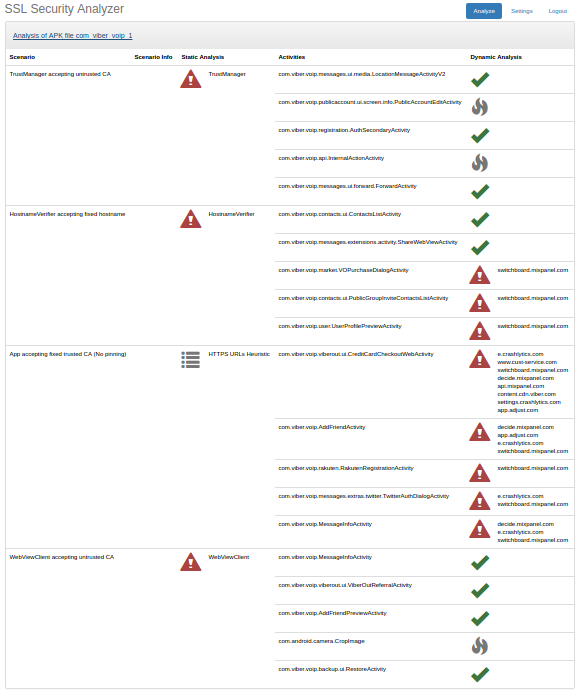
\includegraphics[width=\textwidth,height=1\textheight]{matrix.png}
\end{figure}

\chapter{Summary and future work}

To summarize, a web service for distributed, automatic analysis of APKs for SSL vulnerabilities was developed as part of this thesis. The service allows detection of vulnerable X509TrustManager, HostnameVerifier and WebViewClient implementations and can further detect apps that do not use certificate pinning. It further supports customization of the analysis scenarios to test for more specific threat scenarios.\\
An analysis of 100 apps with this service revealed that 74\% of the apps which could be analysed for certificate pinning did not use the measure. Furthermore, 3 apps had vulnerabilities which allow an attacker to perform a successful Man-In-The-Middle attack against these apps. This shows that insecure use of Android SSL APIs is still an important issue.

Regarding future work, there are some possible improvements and extensions for the Android SSL Analyzer Service. 
Support for analysis guided by manual user input could easily be added for cases where the user has access to the machine running dynamic analysis or if the whole Android SSL Analyzer Service is run on the users machine. This would allow security researchers to perform Man-In-The-Middle attacks on Android apps without having to set up the whole environment that is required.\\
The scripting interface offered by mitmdump could also be used for more than log generation. There is for example a mitmdump script performing SSL Stripping available on the internet \cite{MitmdumpSSLstrip} that could be adjusted and integrated into the Android SSL Analyzer Service.\\
By offering a clearly documented API with results in JSON format instead of only HTML, automated testing with fuzzed certificates or certificates created by combinatorial methods as explained in \cite{Brubaker,Kleine} could be performed in an Android environment.\\
Finally, new static analysis methods supporting additional vulnerability types and entry points could be added and the existing HTTP/S URL Heuristic could be improved.

\let\cleardoublepage\clearpage

\backmatter

% Use an optional list of figures.
% \listoffigures % Starred version, i.e., \listoffigures*, removes the toc entry.

% Use an optional list of tables.
%\cleardoublepage % Start list of tables on the next empty right hand page.
%\listoftables % Starred version, i.e., \listoftables*, removes the toc entry.

% Use an optional list of alogrithms.
% \listofalgorithms
% \addcontentsline{toc}{chapter}{List of Algorithms}

% Add an index.
\printindex

% Add a glossary.
\printglossaries

% Add a bibliography.
\begin{thebibliography}{99}

\bibitem{Adb} Adb.\\\url{https://developer.android.com/studio/command-line/adb.html}, August 2017

\bibitem{Androguard} Androguard. \url{https://github.com/androguard/androguard}, August 2017

\bibitem{AndroidPlatformVersions}
Android platform versions. \url{https://developer.android.com/about/dashboards/index.html#Platform}, August 2017

\bibitem{AndroidViewClient} AndroidViewClient. \url{https://github.com/dtmilano/AndroidViewClient}, August 2017

\bibitem{Android7NetworkSecurityConfig} Android 7.0 Network Security Config. \url{https://developer.android.com/about/versions/nougat/android-7.0.html#network_security_config}, August 2017

\bibitem{Android7Release} Android 7.0 Release. \url{https://blog.google/products/android/android-70-nougat-more-powerful-os-made/}, August 2017

\bibitem{Apktool} Apktool. \url{https://ibotpeaches.github.io/Apktool}, August 2017

\bibitem{Arnbak}Axel Arnbak, Hadi Asghari, Michel Van Eeten and Nico Van Eijk. Security collapse in the HTTPS market. \textit{In Communications of the ACM, 2014, Pages 47 - 55}

\bibitem{Brubaker}C. Brubaker, S. Jana, B. Ray, S. Khurshid and V. Shmatikov. Using Frankencerts for Automated Adversarial Testing of Certificate Validation in SSL/TLS Implementations. \textit{In Proceedings of the 2014 IEEE Symposium on Security and Privacy, 2014, Pages 114 - 129}

\bibitem{Celery} Celery. \url{http://www.celeryproject.org}, August 2017

\bibitem{Conti} Mauro Conti, Nicola Dragoni and Sebastiano Gottardo. MITHYS: Mind The Hand You Shake - Protecting Mobile Devices from SSL Usage Vulnerabilities. \textit{International Workshop on Security and Trust Management, 2013, Pages 65 - 81}

\bibitem{Docker} Docker. \url{https://www.docker.com/what-docker}, August 2017

\bibitem{DockerCompose} Docker compose. \url{https://docs.docker.com/compose}, August 2017

\bibitem{Fahl2012} Sascha Fahl, Marian Harbach, Thomas Muders, Lars Baumg\"{a}rtner, Bernd Freisleben and Matthew Smith. Why Eve and Mallory Love Android: An Analysis of Android SSL (in)Security. \textit{In Proceedings of the 2012 ACM Conference on Computer and Communications Security, 2012, Pages 50 - 61}

\bibitem{Fahl2013} Sascha Fahl, Marian Harbach, Henning Perl, Markus Koetter and Matthew Smith. Rethinking SSL Development in an Appified World. \textit{In Proceedings of the 2013 ACM SIGSAC Conference on Computer \& Communications Security, 2013, Pages 49 - 60}

\bibitem{Flask} Flask. \url{http://flask.pocoo.org}, August 2017

\bibitem{Flask-socketio} Flask-socketio. \url{https://flask-socketio.readthedocs.io/en/latest}, August 2017

\bibitem{Gagnon} Fran{\c{c}}ois Gagnon, Marc-Antoine Ferland, Marc-Antoine Fortier, Simon Desloges, Jonathan Ouellet and Catherine Boileau. AndroSSL: A Platform to Test Android Applications Connection Security. \textit{Foundations and Practice of Security: 8th International Symposium, 2015, Pages 294 - 302}

\bibitem{Georgiev} Martin Georgiev, Subodh Iyengar, Suman Jana, Rishita Anubhai, Dan Boneh and Vitaly Shmatikov. The Most Dangerous Code in the World: Validating SSL Certificates in Non-browser Software. \textit{In Proceedings of the 2012 ACM Conference on Computer and Communications Security, 2012, Pages 38 - 49}

\bibitem{Kleine}K. Kleine and D. E. Simos. Coveringcerts: Combinatorial Methods for X.509 Certificate Testing. \textit{2017 IEEE International Conference on Software Testing, Verification and Validation (ICST), 2017, Pages 69 - 79}

\bibitem{MitmdumpSSLstrip} Mitmdump SSL Stripping.  \url{https://github.com/mitmproxy/mitmproxy/blob/master/examples/complex/sslstrip.py}, August 2017

\bibitem{Mitmproxy} Mitmproxy. \url{https://mitmproxy.org}, August 2017

\bibitem{NetworkSecurityConfig} Network Security Config. \url{https://developer.android.com/training/articles/security-config.html}, August 2017

\bibitem{OkHttp} OkHttp. \url{http://square.github.io/okhttp/}, August 2017

\bibitem{Oltrogge} Marten Oltrogge, Yasemin Acar, Sergej Dechang, Matthew Smith and Sascha Fahl. To Pin or Not to Pin-Helping App Developers Bullet Proof Their TLS Connections. \textit{USENIX Security Symposium, 2015, Pages 239 - 254}

\bibitem{Onwuzurike}Lucky Onwuzurike and Emiliano Cristofaro. Danger is My Middle Name: Experimenting with SSL Vulnerabilities in Android Apps. \textit{Proceedings of the 8th ACM Conference on Security \& Privacy in Wireless and Mobile Networks, 2015, Pages 15}

\bibitem{Pinning} Pinning.\\
\url{https://www.owasp.org/index.php/Certificate_and_Public_Key_Pinning}, August 2017

\bibitem{PinningSymposium} John Kozyrakis. Pinning - Not as simple as it sounds. \textit{Android Security Symposium, 2017, Vienna}, \url{https://usmile.at/sites/default/files/androidsecuritysymposium/presentations2017/Kozyrakis_PinningNotAsSimpleAsItSounds.pdf}, August 2017

\bibitem{RabbitMQ} RabbitMQ. \url{https://www.rabbitmq.com}, August 2017

\bibitem{SMVHunter} SMVHunter. \url{https://github.com/utds3lab/SMVHunter}, August 2017

\bibitem{Sounthiraraj} David Sounthiraraj, Justin Sahs, Garret Greenwood, Zhiqiang Lin and Latifur Khan. Smv-hunter: Large scale, automated detection of ssl/tls man-in-the-middle vulnerabilities in android apps. \textit{In Proceedings of the 21st Annual Network and Distributed System Security Symposium (NDSS’14), 2014}

\bibitem{Tendulkar}Vasant Tendulkar and William Enck. An Application Package Configuration Approach to Mitigating Android SSL Vulnerabilities. \textit{arXiv preprint arXiv:1410.7745, 2014}

\bibitem{Viber} Viber. \url{https://play.google.com/store/apps/details?id=com.viber.voip&hl=de}, August 2017

\bibitem{Zuo} Chaoshun Zuo, Jianliang Wu and Shanqing Guo. Automatically Detecting SSL Error-Handling Vulnerabilities in Hybrid Mobile Web Apps. \textit{Proceedings of the 10th ACM Symposium on Information, Computer and Communications Security, 2015, Pages 591 - 596}

\end{thebibliography}
\end{document}
